\documentclass[14pt,a4paper]{extarticle}
\usepackage{../templates/preamble}
\usepackage{amsmath}

\newcommand{\reportof}{практической работе №7}
\newcommand{\theme}{Вектора и матрицы. Градиент.}

\begin{document}
\begin{titlepage}
    \begin{center}
        {\bfseries
        МИНОБРНАУКИ РОССИИ\par
        САНКТ-ПЕТЕРБУРГСКИЙ ГОСУДАРСТВЕННЫЙ\par
        ЭЛЕКТРОТЕХНИЧЕСКИЙ УНИВЕРСИТЕТ\par
        <<ЛЭТИ>> ИМ. В.И. УЛЬЯНОВА (ЛЕНИНА)\par
        Кафедра \department

        \vspace{0.23\textheight}
        ОТЧЁТ\par
        по \reportof\par
        по дисциплине <<\discipline>>\par
        Тема: \theme
        \vspace{0.28\textheight}
        }
        \begin{table}[!ht]
            \begin{tabularx}{\textwidth}{p{60mm}X>{\centering\arraybackslash}p{45mm}}
                Студент гр. 4352 & \_\_\_\_\_\_\_\_\_\_\_\_\_\_\_\_\_\_\_\_ & {Даричев Е. М.} \\ [5.4mm]  % Line height
                Преподаватель    & \_\_\_\_\_\_\_\_\_\_\_\_\_\_\_\_\_\_\_\_ & {\teacher} \\ [5.4mm]
            \end{tabularx}
        \end{table}

        Санкт-Петербург\par
        \yyear
    \end{center}
\end{titlepage}
\setcounter{page}{2}

\section*{Цель работы}
        Изучить методы работы с частными производными
функций нескольких переменных и научиться вычислять 
MSE функций нескольких переменных.


\section*{Отчёт о проделанной работе}
В первом задании нужно сложить векторы, складывать векторы можно только одной размерности.

1. \[\begin{pmatrix} 1 & 2 & 3 & 4 \end{pmatrix} + \begin{pmatrix} 5 & 6 & 7 & 8 & 9 \end{pmatrix}\]
-- операция невозможна, так как не совпадает количество элементов ($4 \neq 5$);

2. \[\begin{pmatrix} 1 & 2 & 3 & 4 \end{pmatrix} + \begin{pmatrix} 10 & 11 & 12 & 13 \end{pmatrix} = \begin{pmatrix} 11 & 13 & 15 & 17 \end{pmatrix};\]

3. \[\begin{pmatrix} 1 & 2 & 3 & 4 \end{pmatrix} + \begin{pmatrix} 1 \\ 2 \\ 3 \\ 4 \end{pmatrix}\]
-- операция сложения невозможна, так как вектор-строка и вектор-столбец не совместимы;

4. \[\begin{pmatrix} 15 \\ 16 \\ 17 \\ 18 \\ 19 \end{pmatrix} + \begin{pmatrix} 3 \\ 3 \\ 3 \\ 3 \\ 3 \end{pmatrix} = \begin{pmatrix} 18 \\ 19 \\ 20 \\ 21 \\ 22 \end{pmatrix};\]

5. \[\begin{pmatrix} 15 \\ 16 \\ 17 \\ 18 \\ 19 \\ 21 \end{pmatrix} + \begin{pmatrix} 3 \\ 3 \\ 3 \\ 3 \\ 3 \end{pmatrix}\]
-- операция невозможна, так как не совпадает количество элементов ($6 \neq 5$).

Во втором задании нужно найти значения выражений.

1. \[5\times\begin{pmatrix} 1 & 2 & 3 & 4 & 5 & 6 \end{pmatrix}-3\times\begin{pmatrix} 5 & 6 & 7 & 8 & 9 & 10 \end{pmatrix} = \begin{pmatrix} -10 & -8 & -6 & -4 & -2 & 0 \end{pmatrix};\]

2. \[12\times\begin{pmatrix} 7 & 12 & 11 & 14 & 9 & 16 & 21 \end{pmatrix}-3.2\times\begin{pmatrix} 13 & 61 & 24 & 76 & 1 & 3 & 8 \end{pmatrix} =\]
\[=\begin{pmatrix} 42.4 & -51.2 & 55.2 & -75.2 & 104.8 & 182.4 & 226.4 \end{pmatrix};\]

3. \[7\times\begin{pmatrix} 15 \\ 16 \\ 17 \\ 18 \\ 19 \end{pmatrix}+\frac{1}{3}\times\begin{pmatrix} 3 \\ 3 \\ 3 \\ 3 \\ 3 \end{pmatrix}
=\begin{pmatrix} 106 \\ 113 \\ 120 \\ 127 \\ 134 \end{pmatrix};\]

4. \[7\times\begin{pmatrix} 11 \\ 21 \\ 78 \\ 32 \\ 2 \end{pmatrix}-\frac{2}{5}\times\begin{pmatrix} 5 \\ 6 \\ 7 \\ 9 \\ 3 \end{pmatrix}
=\begin{pmatrix} 75 \\ 
    144.6 \\ 
    543.2 \\ 
    220.4 \\ 
    12.8 \end{pmatrix};\]

В третьем задании нужно найти скалярное произведение векторов, если операция имеет смысл.

1. \[\begin{pmatrix} 1 & 2 & 3 & 4 & 5 \end{pmatrix}\cdot\begin{pmatrix} 5 & 6 & 7 & 8 & 9 \end{pmatrix} = 5 + 12 + 21 + 32 + 45 = 115;\]

2. \[\begin{pmatrix} 4 & 3 & 8 & 12 & 1 \end{pmatrix}\cdot\begin{pmatrix} 3 & 2 & 13 & 8 & 5 \end{pmatrix} = 12 + 6 + 104 + 96 + 5 = 223;\]

3. \[\begin{pmatrix} 1 & 2 & 3 & 4 \end{pmatrix}\cdot\begin{pmatrix} 5 & 6 & 7 & 8 & 9 \end{pmatrix}\]
-- векторы нельзя скалярно перемножить, так как у них разная размерность ($4 \neq 5$).

В четвёртом задании нужно транспонировать матрицы. Для нужно их как бы отразить по главной диагонали (поменять строки и столбы местами).

1. Транспонирование вектора-строки:
\[
(5\ 6\ 7\ 8\ 9)^T = \begin{pmatrix} 5 \\ 6 \\ 7 \\ 8 \\ 9 \end{pmatrix};\]
2. Транспонирование вектора-столбца:
\[
\begin{pmatrix}
5 \\
6 \\
7 \\
8 \\
9
\end{pmatrix}^T = (5\ 6\ 7\ 8\ 9);\]
3. Транспонирование матрицы $4\times4$:
\[
\begin{pmatrix}
1 & 2 & 3 & 4 \\
5 & 6 & 7 & 8 \\
9 & 10 & 11 & 12 \\
13 & 14 & 15 & 16
\end{pmatrix}^T = 
\begin{pmatrix}
1 & 5 & 9 & 13 \\
2 & 6 & 10 & 14 \\
3 & 7 & 11 & 15 \\
4 & 8 & 12 & 16
\end{pmatrix};
\]

Транспонирование матрицы можно запрограммировать с помощью sympy (рис. \ref{pic:trans}).

\begin{figure}[h!]
    \centering
    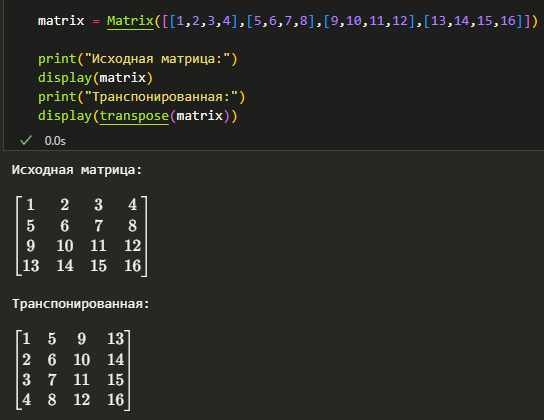
\includegraphics[width=0.7\textwidth]{figures/transp.png}
    \caption{Нахождение транспонированной матрицы}
    \label{pic:trans}
\end{figure}

Для транспонирования матрицы нужно написать код, в котором
функция будет принимать и возвращать либо numpy.array, либо list (рис. \ref{pic:code}).
\begin{figure}[h!]
    \centering
    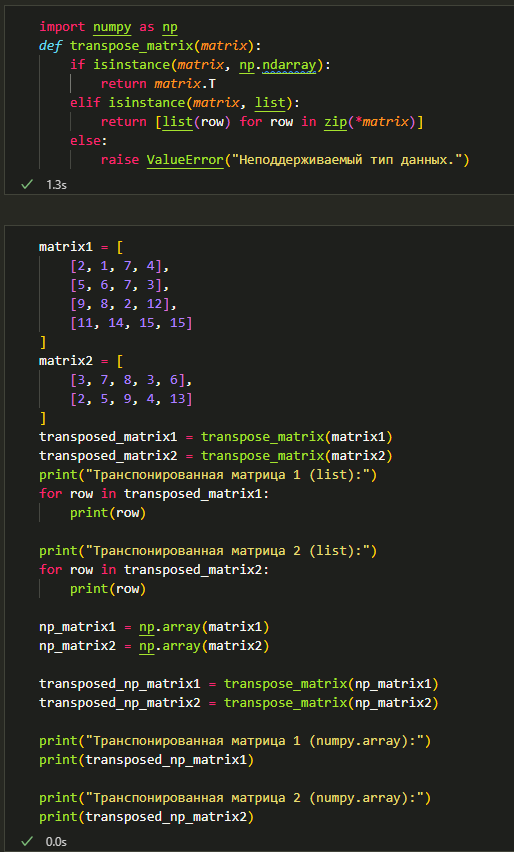
\includegraphics[width=0.49\textwidth]{figures/transp_code.png}
    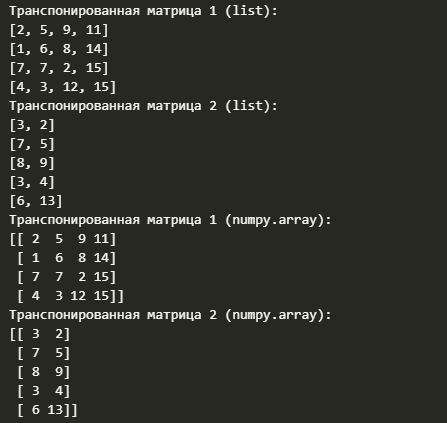
\includegraphics[width=0.49\textwidth]{figures/transp_result.png}
    \caption{Транспонирование матриц}
    \label{pic:code}
\end{figure}

В последнем задании нужно завершить градиентный спуск,
начатый в методических материалах. Движение будет происходить в направлении антиградиента,
размер шага равен $0.01$. В каждой новой точке антиградиент будет разным. Нужно добиться величины MSE меньше 6,36,
а также посчитать количество шагов градиентного спуска.

Функция потерь MSE:
\[{MSE}(a_1, a_2) = \frac{1}{4} ((a_1 + 2a_2 - 5)^2 + (5a_1 + 3a_2 - 6)^2 +\]\[+ (2a_1 + 4a_2 - 10)^2 +(3a_1 + 7a_2 - 8)^2).\]

Градиент MSE:
\[\nabla \text{MSE}(a_1, a_2) = \begin{pmatrix}19.5a_1 + 23a_2 - 39.5 \\ 23a_1 + 39a_2 - 62\end{pmatrix}.\]

Начальная точка: $(a_1, a_2) = (0.57, 0.91).$

Начальное значение MSE: $8.56.$

Вычисляем новое значение MSE (рис. \ref{pic:mse}). Значение меньше $6.36$ было достигнуто за 6 шагов.

\begin{figure}[h!]
    \centering
    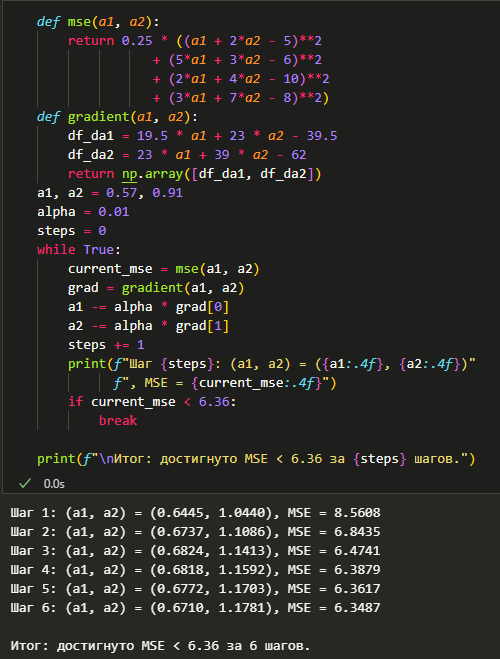
\includegraphics[scale=0.7]{figures/mse.png}
    \caption{Поиск градиента меньшего $6.36$}
    \label{pic:mse}
\end{figure}

\section*{Вывод.}

В ходе работы были изучены частные производные функции нескольких переменных,
а также метод нахождения среднеквадратичной ошибки для таких функций.

\end{document}